% Options for packages loaded elsewhere
\PassOptionsToPackage{unicode}{hyperref}
\PassOptionsToPackage{hyphens}{url}
%
\documentclass[
]{article}
\usepackage{lmodern}
\usepackage{amssymb,amsmath}
\usepackage{ifxetex,ifluatex}
\ifnum 0\ifxetex 1\fi\ifluatex 1\fi=0 % if pdftex
  \usepackage[T1]{fontenc}
  \usepackage[utf8]{inputenc}
  \usepackage{textcomp} % provide euro and other symbols
\else % if luatex or xetex
  \usepackage{unicode-math}
  \defaultfontfeatures{Scale=MatchLowercase}
  \defaultfontfeatures[\rmfamily]{Ligatures=TeX,Scale=1}
\fi
% Use upquote if available, for straight quotes in verbatim environments
\IfFileExists{upquote.sty}{\usepackage{upquote}}{}
\IfFileExists{microtype.sty}{% use microtype if available
  \usepackage[]{microtype}
  \UseMicrotypeSet[protrusion]{basicmath} % disable protrusion for tt fonts
}{}
\makeatletter
\@ifundefined{KOMAClassName}{% if non-KOMA class
  \IfFileExists{parskip.sty}{%
    \usepackage{parskip}
  }{% else
    \setlength{\parindent}{0pt}
    \setlength{\parskip}{6pt plus 2pt minus 1pt}}
}{% if KOMA class
  \KOMAoptions{parskip=half}}
\makeatother
\usepackage{xcolor}
\IfFileExists{xurl.sty}{\usepackage{xurl}}{} % add URL line breaks if available
\IfFileExists{bookmark.sty}{\usepackage{bookmark}}{\usepackage{hyperref}}
\hypersetup{
  pdftitle={Auto-generated report from BCEA},
  hidelinks,
  pdfcreator={LaTeX via pandoc}}
\urlstyle{same} % disable monospaced font for URLs
\usepackage[margin=1in]{geometry}
\usepackage{graphicx,grffile}
\makeatletter
\def\maxwidth{\ifdim\Gin@nat@width>\linewidth\linewidth\else\Gin@nat@width\fi}
\def\maxheight{\ifdim\Gin@nat@height>\textheight\textheight\else\Gin@nat@height\fi}
\makeatother
% Scale images if necessary, so that they will not overflow the page
% margins by default, and it is still possible to overwrite the defaults
% using explicit options in \includegraphics[width, height, ...]{}
\setkeys{Gin}{width=\maxwidth,height=\maxheight,keepaspectratio}
% Set default figure placement to htbp
\makeatletter
\def\fps@figure{htbp}
\makeatother
\setlength{\emergencystretch}{3em} % prevent overfull lines
\providecommand{\tightlist}{%
  \setlength{\itemsep}{0pt}\setlength{\parskip}{0pt}}
\setcounter{secnumdepth}{-\maxdimen} % remove section numbering
\usepackage{graphicx} \usepackage{bm}

\title{Auto-generated report from BCEA}
\author{}
\date{\vspace{-2.5em}Version: 27 August, 2020}

\begin{document}
\maketitle

\hypertarget{cost-effectiveness-analysis}{%
\subsection{Cost-effectiveness
analysis}\label{cost-effectiveness-analysis}}

The cost-effectiveness analysis is based on the maximisation of the
expected utility, defined as the \emph{monetary net benefit}
\(nb_t=ke_t-c_t\). Here \(t\) indicates one of the interventions
(treatments) being assessed, while \((e,c)\) indicate the relevant
measures of \emph{effectiveness} and \emph{cost}. For each intervention,
the expected utility is computed as
\(\mathcal{NB}_t=k\mbox{E}[e_t]-\mbox{E}[c_t]\). When comparing two
interventions (say, \(t=1\) vs \(t=0\)), or using a pairwise comparison,
we can determine the ``best'' alternative by considering the difference
in the expected utilities \(\mbox{EIB}=\mathcal{NB}_1-\mathcal{NB}_0\).
This can also be expressed in terms of the \emph{population
effectiveness and cost differentials}
\(\mbox{EIB}=k\mbox{E}[\Delta_e]-\mbox{E}[\Delta_c]\), where
\(\Delta_e=\mbox{E}[e\mid\bm\theta_1]-\mbox{E}[e\mid\bm\theta_0]\) and
\(\Delta_c=\mbox{E}[c\mid\bm\theta_1]-\mbox{E}[c\mid\bm\theta_0]\) are
the average effectiveness and cost, as function of the relevant model
parameters \(\bm\theta=(\bm\theta_0,\bm\theta_1)\).

This sub-section presents a summary table reporting basic economic
results as well as the optimal decision, given the selected
willingness-to-pay threshold \(k=20100\). The table below presents a
summary of the optimal decision, as well as the values of the Expected
Incremental Benefit
\(\mbox{EIB}=k\mbox{E}[\Delta_e]-\mbox{E}[\Delta_c]\),
Cost-Effectiveness Acceptability Curve
\(\mbox{CEAC}=\Pr(k\Delta_e-\Delta_c)\) and Incremental
Cost-Effectiveness Ratio
\(\mbox{ICER}=\displaystyle\frac{\mbox{E}[\Delta_c]}{\mbox{E}[\Delta_e]}\),
for the set willingness-to-pay value.

\begin{verbatim}

Cost-effectiveness analysis summary 

Reference intervention:  intervention 2
Comparator intervention: intervention 1

Optimal decision: choose intervention 1 for k < 20100 and intervention 2 for k >= 20100


Analysis for willingness to pay parameter k = 20100

               Expected utility
intervention 1          -36.054
intervention 2          -34.826

                                    EIB  CEAC  ICER
intervention 2 vs intervention 1 1.2284 0.529 20098

Optimal intervention (max expected utility) for k = 20100: intervention 2
           
EVPI 3.0287
\end{verbatim}

\hypertarget{cost-effectiveness-plane}{%
\subsection{Cost-effectiveness plane}\label{cost-effectiveness-plane}}

The following graph shows the \emph{cost-effectiveness plane}. This
presents the joint distribution of the population average benefit and
cost differential, \((\Delta_e,\Delta_c)\) and can be used to assess the
uncertainty underlying the decision-making problem.

Each point in the graph represents a `potential future' in terms of
expected incremental economic outcomes. The shaded portion of the plane
is the \emph{`sustainability area'}. The more points lay in the
sustainability area, the more likely that the reference intervention
will turn out to be cost-effective, at a given willingness to pay
threshold, \(k\) (in this case selected at \(k=\) 20100).

\begin{center}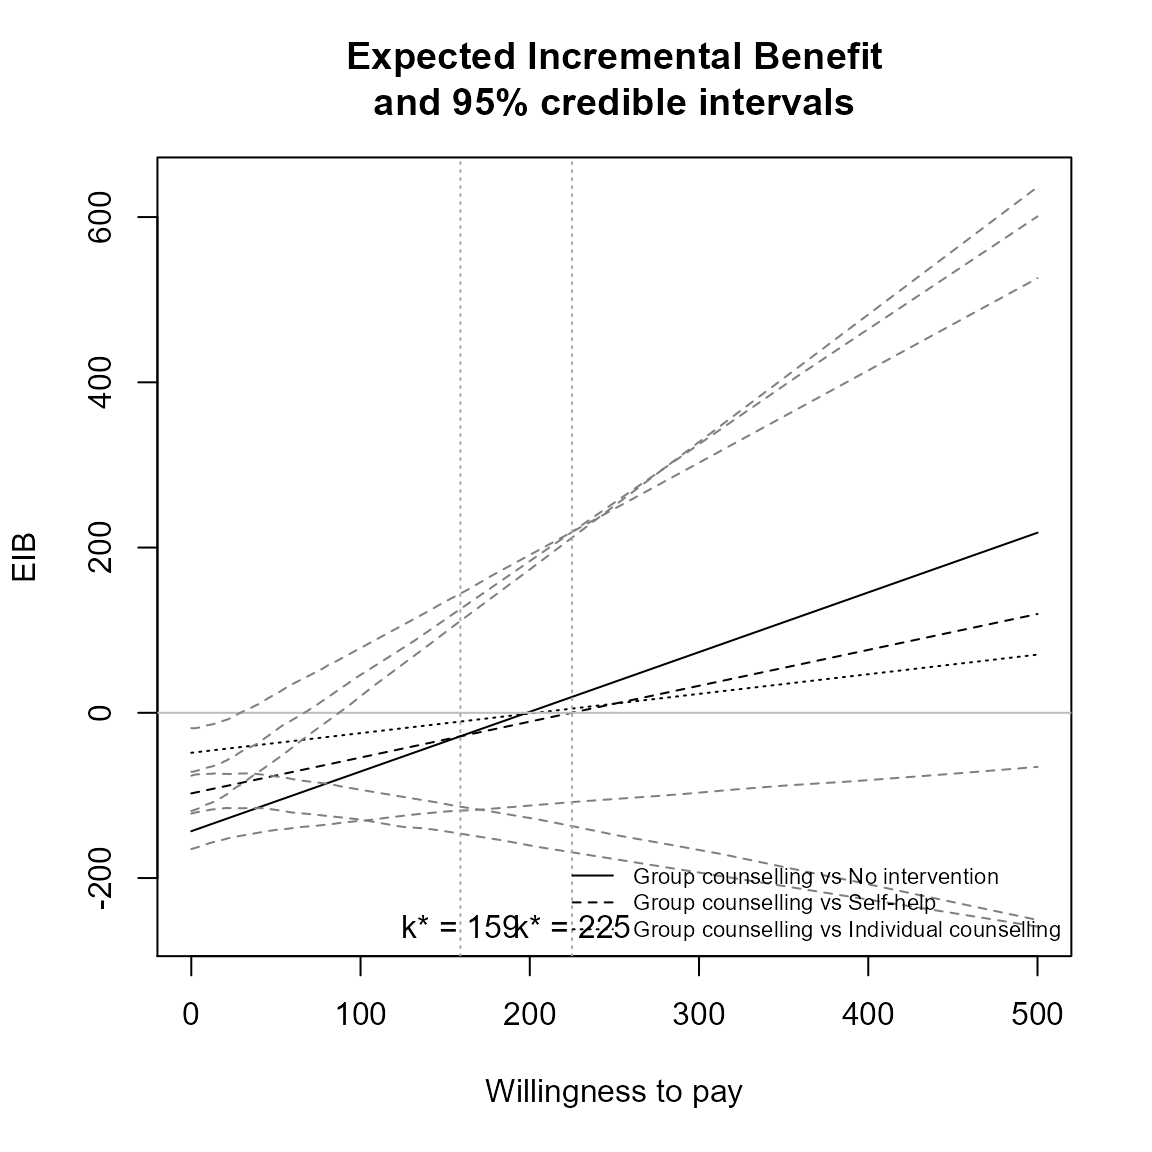
\includegraphics{report_files/figure-latex/unnamed-chunk-10-1} \end{center}

\hypertarget{expected-incremental-benefit}{%
\subsection{Expected Incremental
Benefit}\label{expected-incremental-benefit}}

The following graph shows the \emph{Expected Incremental Benefit} (EIB),
as a function of a grid of values for the willingness to pay \(k\) (in
this case in the interval 0 - 50000).

The EIB can be directly linked with the decision rule applied to the
ICER. If a willingness to pay value \(k^*\) exists in correspondence of
which \(\mbox{EIB}=0\) this value of \(k\) is called the
\emph{break-even point}. It corresponds to the maximum uncertainty
associated with the decision between the two comparators, with equal
expected utilities for the two interventions. In other terms, for two
willingness to pay values, one greater and one less than \(k^*\), there
will be two different optimal decisions. The graph also reports the 95\%
credible limits around the EIB.

\begin{center}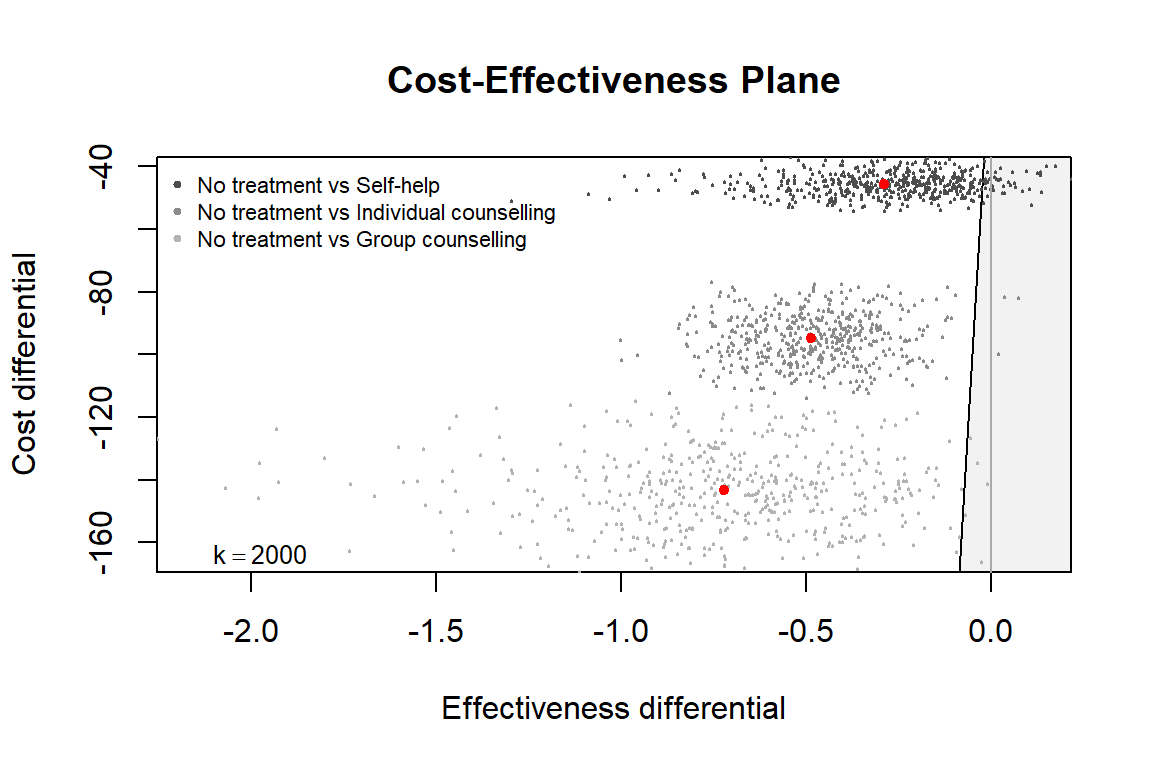
\includegraphics{report_files/figure-latex/unnamed-chunk-11-1} \end{center}

\hypertarget{cost-effectiveness-acceptability-curve}{%
\subsection{Cost-effectiveness acceptability
curve}\label{cost-effectiveness-acceptability-curve}}

The \emph{Cost-Effectiveness Acceptability Curve} (CEAC) estimates the
probability of cost-effectiveness, for different willingness to pay
thresholds. The CEAC is used to evaluate the uncertainty associated with
the decision-making process, since it quantifies the degree to which a
treatment is preferred. This is measured in terms of the difference in
utilities, normally the incremental benefit. Effectively, the CEAC
represents the proportion of simulations in which \(t=1\) is associated
with a higher utility than \(t=0\).

The following graph shows the cost-effectiveness acceptability curve
(CEAC). The CEAC represents the proportion of `potential futures' in
which the reference intervention is estimated to be more cost-effective
than the comparator. Thus, it can be interpreted as the `probability of
cost-effectiveness'.

\begin{center}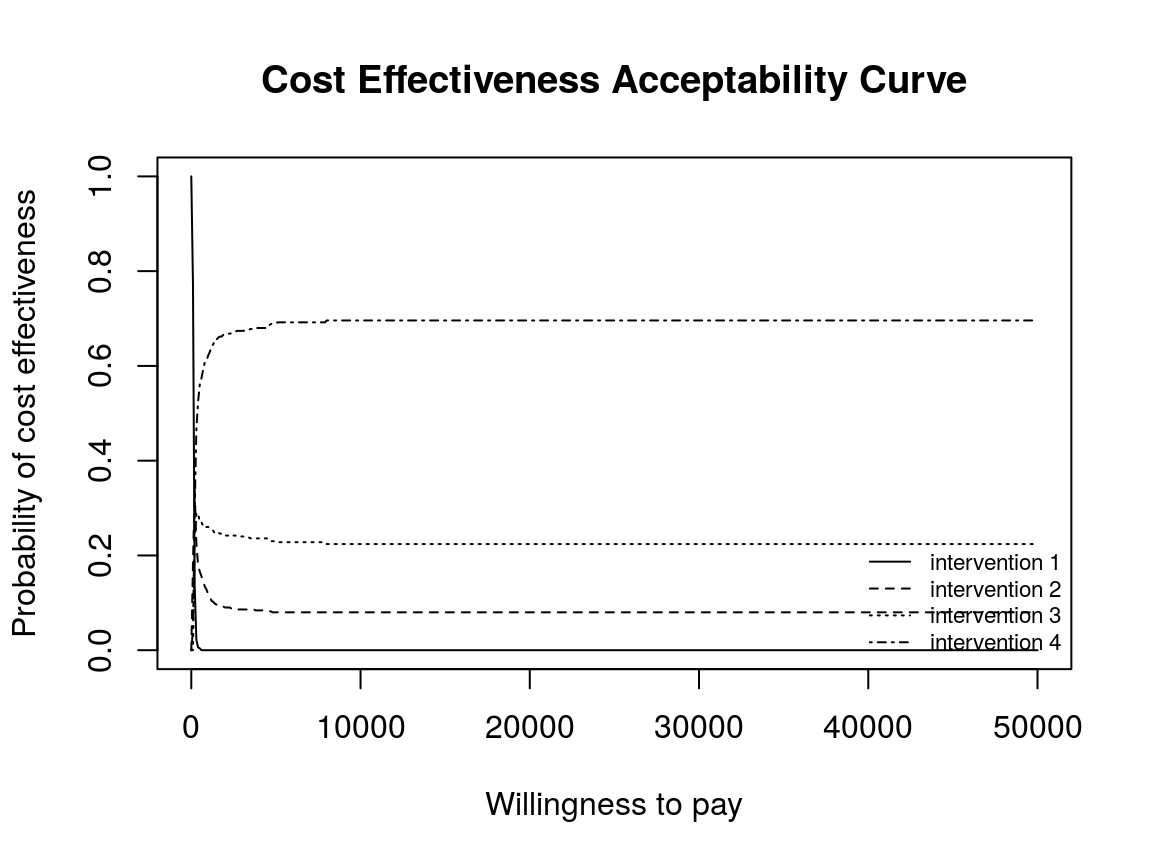
\includegraphics{report_files/figure-latex/unnamed-chunk-12-1} \end{center}

\hypertarget{cost-effectiveness-acceptability-frontier}{%
\subsection{Cost-effectiveness acceptability
frontier}\label{cost-effectiveness-acceptability-frontier}}

In addition to the CEAC, we can also visualise the uncertainty in the
decision-making process using the \emph{Cost-Effectiveness Acceptability
Frontier} (CEAF). The frontier is defined as the maximum value of the
probability of cost-effectiveness among all comparators. It is an
indication of the uncertainty associated with choosing the cost
effective intervention. In other terms, higher frontier values
correspond to lower decision uncertainty.

\begin{center}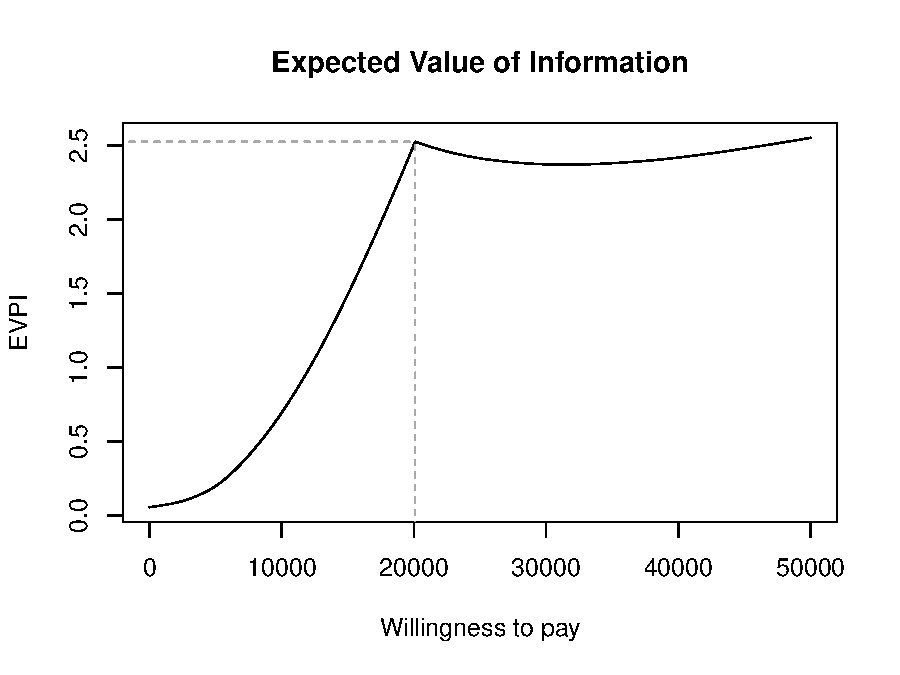
\includegraphics{report_files/figure-latex/unnamed-chunk-13-1} \end{center}

\hypertarget{cost-effectiveness-acceptability-frontier-1}{%
\subsection{Cost-effectiveness acceptability
frontier}\label{cost-effectiveness-acceptability-frontier-1}}

In addition to the CEAC, we can also visualise the uncertainty in the
decision-making process using the \emph{Cost-Effectiveness Acceptability
Frontier} (CEAF). The frontier is defined as the maximum value of the
probability of cost-effectiveness among all comparators. It is an
indication of the uncertainty associated with choosing the cost
effective intervention. In other terms, higher frontier values
correspond to lower decision uncertainty.

\begin{center}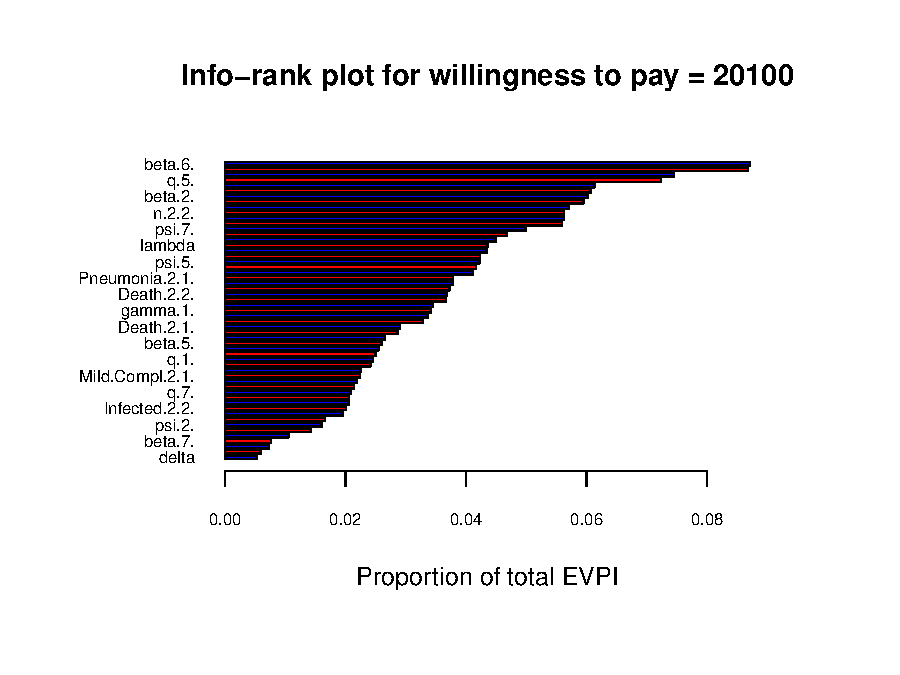
\includegraphics{report_files/figure-latex/unnamed-chunk-14-1} \end{center}

\hypertarget{cost-effectiveness-efficiency-frontier}{%
\subsection{Cost-effectiveness efficiency
frontier}\label{cost-effectiveness-efficiency-frontier}}

The \emph{Cost-Effectiveness Efficiency Frontier} (CEEF) compares the
net costs and benefits of different interventions in a given therapeutic
area. It is different from the common differential approach (e.g.~based
on the Cost-Effectiveness plane), because it is based on the \emph{net}
measures. The predicted costs and effectiveness for the interventions
under consideration are compared directly to the costs and effectiveness
for the treatments that are currently available. The frontier in itself
defines the set of interventions for which cost is at an acceptable
level for the benefits given by the treatment. A new intervention is
\emph{efficient} if its average effectiveness is greater than any of the
currently available alternatives, or its cost are lower than that
associated with other interventions of the same effectiveness.

In the following plot, the circles indicate the mean for the cost and
effectiveness distributions for each treatment option. The number in
each circle corresponds to the order of the treatments in the legend. If
the number is black then the intervention is on the efficiency frontier.
Grey numbers indicate dominated treatments.

\begin{verbatim}

Cost-effectiveness efficiency frontier summary 

Interventions on the efficiency frontier:
               Effectiveness   Costs Increase slope Increase angle
intervention 1   -0.00105595  9.6555             NA             NA
intervention 2   -0.00080537 14.6914          20098         1.5707
\end{verbatim}

\begin{center}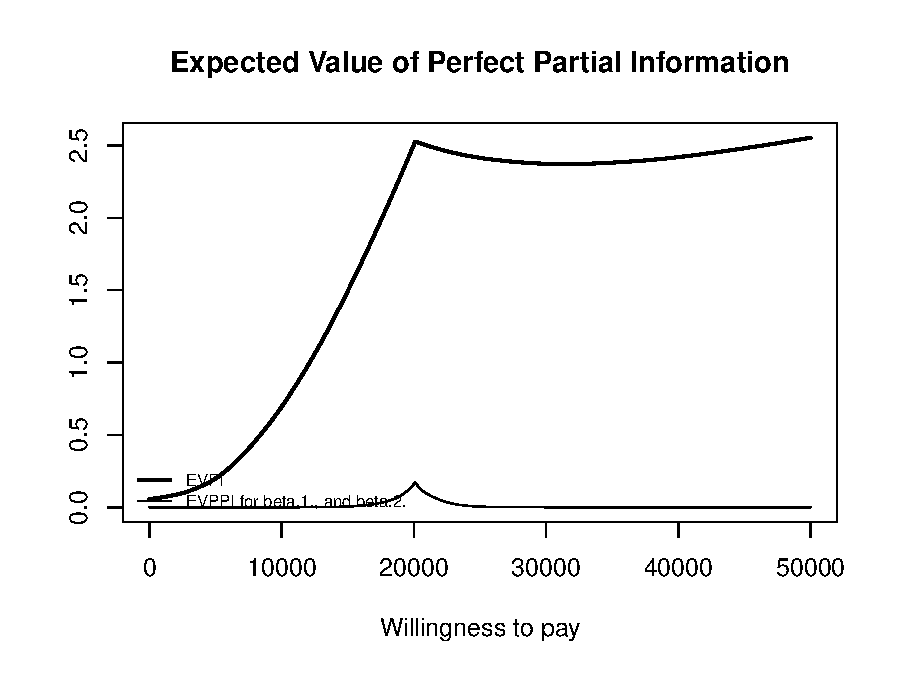
\includegraphics{report_files/figure-latex/unnamed-chunk-15-1} \end{center}

The summary is composed of two tables, reporting information for the
comparators included on the frontier. It also details the average health
effects and costs for the comparators not on the frontier, if any. For
the interventions included on the frontier, the slope of the frontier
segment connecting the intervention to the previous efficient one and
the angle inclination of the segment (with respect to the \(x-\)axis),
measured in radians, are also reported. In particular, the slope can be
interpreted as the increase in costs for an additional unit in
effectiveness, i.e.~the ICER for the comparison against the previous
treatment.

The dominance type for comparators not on the efficiency frontier is
reported in the output table. This can be of two types: absolute or
extended dominance. An intervention is absolutely dominated if another
comparator has both lower costs and greater health benefits, i.e.~the
ICER for at least one pairwise comparison is negative. Comparators in a
situation of extended dominance are not wholly inefficient, but are
dominated because a combination of two other interventions will provide
more benefits for lower costs.

\hypertarget{expected-value-of-perfect-information}{%
\subsection{Expected value of perfect
information}\label{expected-value-of-perfect-information}}

One measure to quantify the value of additional information is known as
the \emph{Expected Value of Perfect Information} (EVPI). This measure
translates the uncertainty associated with the cost-effectiveness
evaluation in the model into an economic quantity. This quantification
is based on the \emph{Opportunity Loss} (OL), which is a measure of the
potential losses caused by choosing the most cost-effective intervention
\emph{on average} when it does not result in the intervention with the
highest utility in a `possible future'. A future can be thought of as
obtaining enough data to know the exact value of the utilities for the
different interventions. This would allow the decision makers to known
the optimal treatment with certainty. The opportunity loss occurs when
the optimal treatment on average is non-optimal for a specific point in
the distribution for the utilities.

To calculate the EVPI practically, possible futures for the different
utilities are represented by the simulations. The utility values in each
simulation are assumed to be known, corresponding to a possible future,
which could happen with a probability based on the current available
knowledge included in and represented by the model. The opportunity loss
is the difference between the maximum value of the simulation-specific
(known-distribution) utility
\(\mbox{NB}^*(\bm\theta)=k\Delta_e-\Delta_c\) and the utility for the
intervention resulting in the overall maximum expected utility
\(\mbox{NB}(\bm\theta^\tau)\), where
\(\tau=\text{arg max}_t ~\mathcal{NB}^t\).

Usually, for a large number simulations the OL will be 0 as the optimal
treatment on average will also be the optimal treatment for the majority
of simulations. This means that the opportunity loss is always positive
as either we choose the current optimal treatment or the treatment with
a higher utility value for that specific simulation. The EVPI is then
defined as the average of the opportunity loss. This measures the
average potential losses in utility caused by the simulation specific
optimal decision being non-optimal in reality.

If the probability of cost-effectiveness is low then more simulations
will give a non-zero opportunity loss and consequently the EVPI will be
higher. This means that if the probability of cost-effectiveness is very
high, it is unlikely that more information would be worthwhile, as the
most cost-effective treatment is already evident. However, the EVPI
gives additional information over the EVPI as it takes into account the
opportunity lost as well as simply the probability of
cost-effectiveness.

For example, there may be a setting where the probability of
cost-effectiveness is low, so the decision maker believes that decision
uncertainty is important. However, this is simply because the two
treatments are very similar in both costs and effectiveness. In this
case the OL will be low as the utilities will be similar for both
treatments for all simulations. Therefore, the cost of making the
incorrect decision is very low. This will be reflected in the EVPI but
not in the CEAC and implies that the optimal treatment can be chosen
with little financial risk, even with a low probability of
cost-effectiveness.

\begin{center}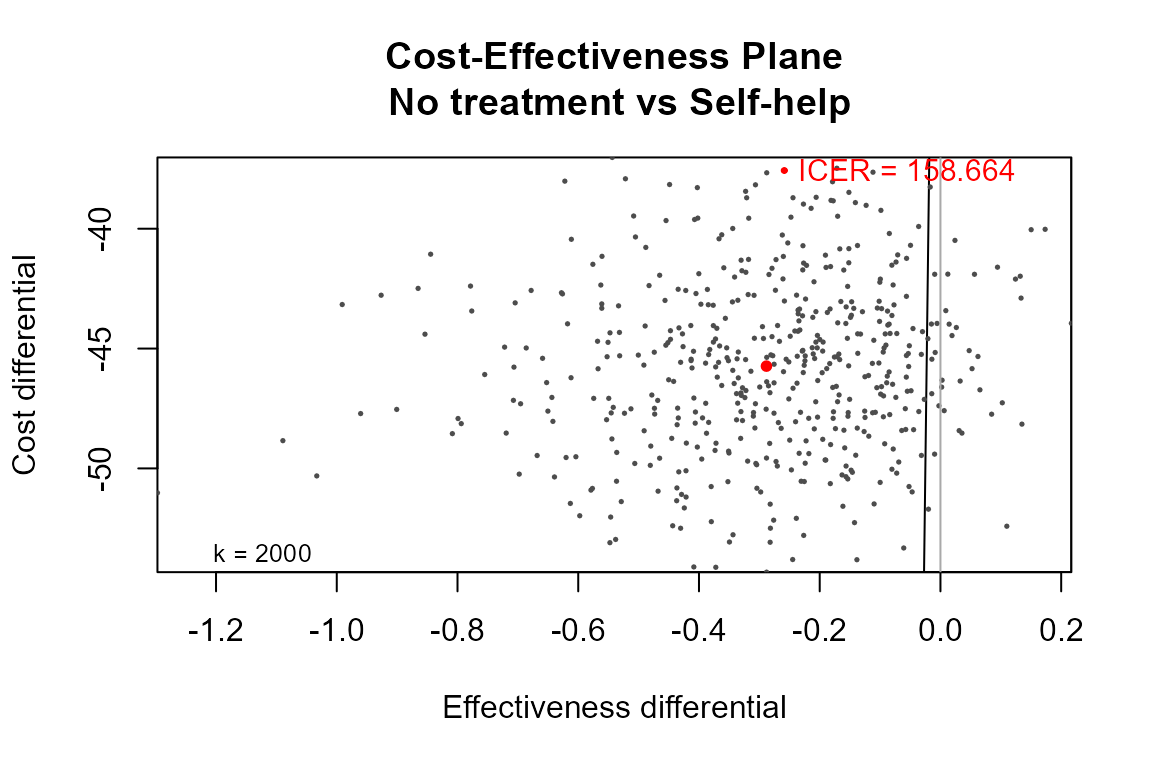
\includegraphics{report_files/figure-latex/unnamed-chunk-16-1} \end{center}

\hypertarget{references}{%
\subsection*{References}\label{references}}
\addcontentsline{toc}{subsection}{References}

\hypertarget{refs}{}
\leavevmode\hypertarget{ref-Baioetal:2017}{}%
Baio, G, A Berardi, and A Heath. 2017. \emph{Bayesian Cost-Effectiveness
Analysis with the R package BCEA}. New York, NY: Springer.
\url{https://doi.org/10.1007/978-3-319-55718-2}.

\end{document}
